\chapter{Evaluation in simulated Data Center Network}\label{ch4}
The last chapter of this work is the evaluation of our proposal in a packet network. We configured a DCN network in a simulated environment, where now the protocol stack is fully implemented. We worked with the open-source discrete event simulator OMNeT++ \cite{omnetpp} and the INET library \cite{inet}, which provides readily deployable components for the TCP/IP stack, link layer and physical layer protocol implementations, as well as models for QoS provisioning. In order to test spatial diversity we extended and customized some of the library components. The most relevant among of these modifications will be reported in this chapter to allow easy reproducibility. Indeed, we dedicate the first section (\S \ref{sec:opp-setup}) to an in-depth description of the simulation methodology and the configuration of the network components and their interactions. Then, we will analyze the results and draw the final conclusions. 
\section{Simulator setup}
\label{sec:opp-setup}
OMNeT++ is a discrete-event simulator, based on message passing. Essentially, the events are represented by messages which are stored in a priority queue. The user can schedule events by creating a message with associated a timestamp, which indicates the moment in time when events need to be simulated and corresponds to the message priority in the queue.  The events are sorted in ascending order of timestamps.  Obviously, there isn't correspondence with the real time, instead all timestamps refer to a simulated time. Therefore, all events are executed at CPU speed and the virtual simulation time is set artificially to the timestamp of the last event popped from the queue. \\ OMNeT++ separates the definition of the model components from their actual implementation. It provides a descriptive language to define which components to include in the simulation model and possibly to define interconnection among them. The interconnections allow different modules to communicate with message passing. Separately, the user can implement the actual behavior of such components. For each of them it is possible to customize the routines to handle events, schedule new events and pass messages to other modules.

We worked in Ubuntu 16.04 environment, using OMNeT++ v.5.2.1 and INET v3.6.4. 
The goal of this section is to explain the setup we used on our simulator and provide implementation details, eventually useful for hands-on experiments with this system. 
\subsection{Traffic generation}
We consider a standard leaf and spine Ethernet-based topology, with only two layers. All hosts in the topology are directly connected through a single 1Gbps links to ToR switches, that comprises the first layer. Then, all ToRs are connected to all spines (second layer), forming a bi-partite graph structure. Also these links are configured at 1Gbps speed. We do not apply any over-subscription, therefore the aggregate bandwidth of all access links equals the bisection bandwidth. The topology and the nomenclature is shown in Fig. \ref{label}.
\begin{figure}
	\centering
	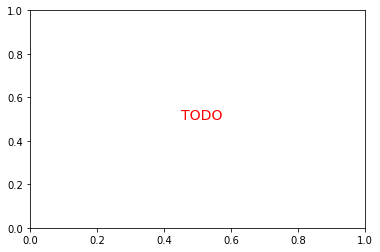
\includegraphics[width=0.5\textwidth]{Chapter3/Figures/todored}
	\caption{Data center topology used in simulations}
\end{figure}%
\\The first point is to generate a given amount of traffic. We want the hosts to fed the DCN with a given offered load $\rho$ defined as the average traffic offered to the switching fabric normalized to the bisection bandwidth. All hosts in the network have a single traffic source application and a single traffic sink application. Flows arrive at traffic sources according to a Poisson process with intensity $\lambda$ and are sent to a traffic sink belonging to another server chosen uniformly at random. Every new flow size is drawn from a given distribution. The flow size distributions that we considered are generally the ones already presented in section \ref{sec:workloads}. We did few experiments also with the uniform distribution at the very beginning to verify what happens when the flow size distribution has low variability. We never accounted for cases of heterogeneous workloads across the data center, thus all servers are always assumed to run the same workload. The bounded Pareto distribution wasn't available by default in the OMNeT++ library. However, it is easy to generate new samples of a random variable $X$ from any distribution through the CDF inversion technique. It is first extracted a uniform point $y \in [0,1]$. The uniform distribution is readily provided in the library of the simulator. Then, the following transformation involving the inverse of the cumulative function $F(x)$ is performed:
\[
x = F^{-1}(y)
\]
Essentially, the value $y$ is projected through $F(x)$ on the support of the distribution, giving the corresponding $y$-th quantile $x$, which is the new realization of the distribution of $X$ we needed. For the bounded Pareto with support in the interval $[u,t]$, whose $F(x)$ has been expressed in Eq.\ref{eq:bpcdf}, it holds:
\[
F^{-1}(y) = \sqrt{-\dfrac{(ut)^\alpha}{yt^\alpha - yu^\alpha - t^\alpha}}
\]
In order to implement the Poisson arrival process it has to be derived its intensity $\lambda$. Let $n_S$ be the number of spines, $n_T$ the number of ToRs and $n_H$ the number of hosts per rack. Denote with $C$ the link capacity connecting a rack with a spine. It has to be expressed the total traffic on the bisection bandwidth as a function of $\lambda$. First write the probability that a flow originated by a server in rack $T_i$ is destined to another server in a rack $T_j$ with $i \neq j$ (exit rack probability):
\[
P_{out} = \frac{(n_T-1)\times n_H}{n_T \times n_H - 1}
\]
Indeed there are $(n_T-1)\times n_H$ possible destinations among the total number of servers, excluded the source. If only cross-rack flows are simulated, obviously $P_{out}$=1.  Next, from the average flow size at application layer $\mathbb{E}[X_{(7)}]=\mathbb{E}[X]$ we need to obtain the average flow size at physical layer $\mathbb{E}[X_{(1)}]$. Define $\mathcal{H}(i)$ the procotol control information (PCI) added by the $i$-th OSI layer. The average flow size at physical layer is the average flow size at application layer with the addition of all headers in between. For a fixed packet size $pktsize$, that we always set to the Maximum Transmission Unit for the Ethernet ($pktsize$=1500B):
\[
\mathbb{E}[X_{(1)}] = \mathbb{E}[X_{(7)}] + \dfrac{\sum_{i=0}^{4}\mathcal{H}(i)}{pktsize}
\]
Since the all racks have the same workload, the total load $\rho$ on the fabric corresponds to the average traffic outgoing a single ToR.
\begin{equation}
	\label{eq:udp-load-generation}
	\rho = \dfrac{\lambda \; n_H \; \mathbb{E}[X_{(1)}]}{n_S \; C} P_{out}
\end{equation} 
Here it has been implicitly used the merging property of independent Poisson processes (PP), that states that merging multiple independent PP gives another PP with rate equal to the sum of individual rates. Inverting Eq.\eqref{eq:udp-load-generation} gives the final intensity $\lambda$ to be adopted by all hosts in the network: 
\begin{equation}
	\label{eq:lambda}
	\lambda = \frac{\rho \; n_S \; C}{n_H \; \mathbb{E}[X_{(1)}] \; P_{out}}
\end{equation}
We performed experiments both with TCP and UDP. The reasons will be explained in details when describing their setup. However, in writing the total traffic with Eq.\eqref{eq:udp-load-generation} it has to be accounted also for control packets of the TCP connections. We decided to disregard \texttt{SYN} and \texttt{FIN} packets, since they really have a negligible impact on the total traffic.  Instead, we considered \texttt{ACK} responses. All hosts of a rack send back an \texttt{ACK} in exchange of every received TCP packet, thus:
\begin{equation}
	\rho_{TCP} = \rho + \gamma \; \rho, \qquad \gamma = \dfrac{acksize}{pktsize}
\end{equation}
The same reasoning applies also if the delayed-ACK option of TCP is applied, but $\gamma$ must be rescaled accordingly.  \\
\subsubsection{Simulation length}
Once $\lambda$ is known, it is possible to derive the simulation time $t_M$ required to observe an average total number of flows $M$:
\[
t_s = \dfrac{1}{\lambda}\;\frac{M}{n_H \; n_T}
\]
The rough criterion we used for choosing $M$ is to tune its value depending on the tail of the flow size distribution and the "importance" of tail flows for the total load. In particular, we considered the mass-weighted function (\S \ref{sec:workloads} Fig. \ref{fig:mwf}) to understand how much traffic is carried by flow sizes corresponding to high percentiles. For instance, for both Pareto distributions we have seen that flow sizes corresponding to percentiles as high as 99-th still carry a lot of traffic (for data mining actually they carry almost all the traffic). Therefore, for these distributions unfortunately we should observe some amount of these tail flows to get the average load $\rho$ that we impose. In this respect, they are important to be simulated. For example, let's suppose we decided --- by looking at the mass-weighted function --- that we want simulate at least 100 realizations of the largest 1\% flows. We need $M \ge 100 \mslash 0.01 = 10000$. Usually for the web search Pareto workload we used $M \sim O(10^{4})$. Note that another aspect to keep in mind is also the number of simulated flows per server, that is the ratio $M \mslash (n_H \; n_T)$. If the topology is very large, the total number of flows $M$ must be increased to avoid non-homogeneity across servers in the offered traffic. For this reasons, the data mining workload it is really not practical and often it has been ignored. 
\subsection{Host configuration}
\label{sec:host-config}
All hosts in the network have one source client application, that generates flows according to the Poisson process, and one sink server application, that only receives flows in order to measure FCT, then discards their bytes. The host configuration changes a bit depending on whether we used TCP or UDP as transport. We run experiments with TCP and UDP, motivated by the noticeable difference among PS and FIFO discipline we observed in chapter \ref{ch:numerical-simulator} for SD-MLFQ. Indeed, the setting adopted for UDP at end hosts turned out to resemble the FIFO service discipline. 
\subsubsection{TCP}
\begin{figure}[!tb]
	\centering
	\captionsetup{width=.75\linewidth}
	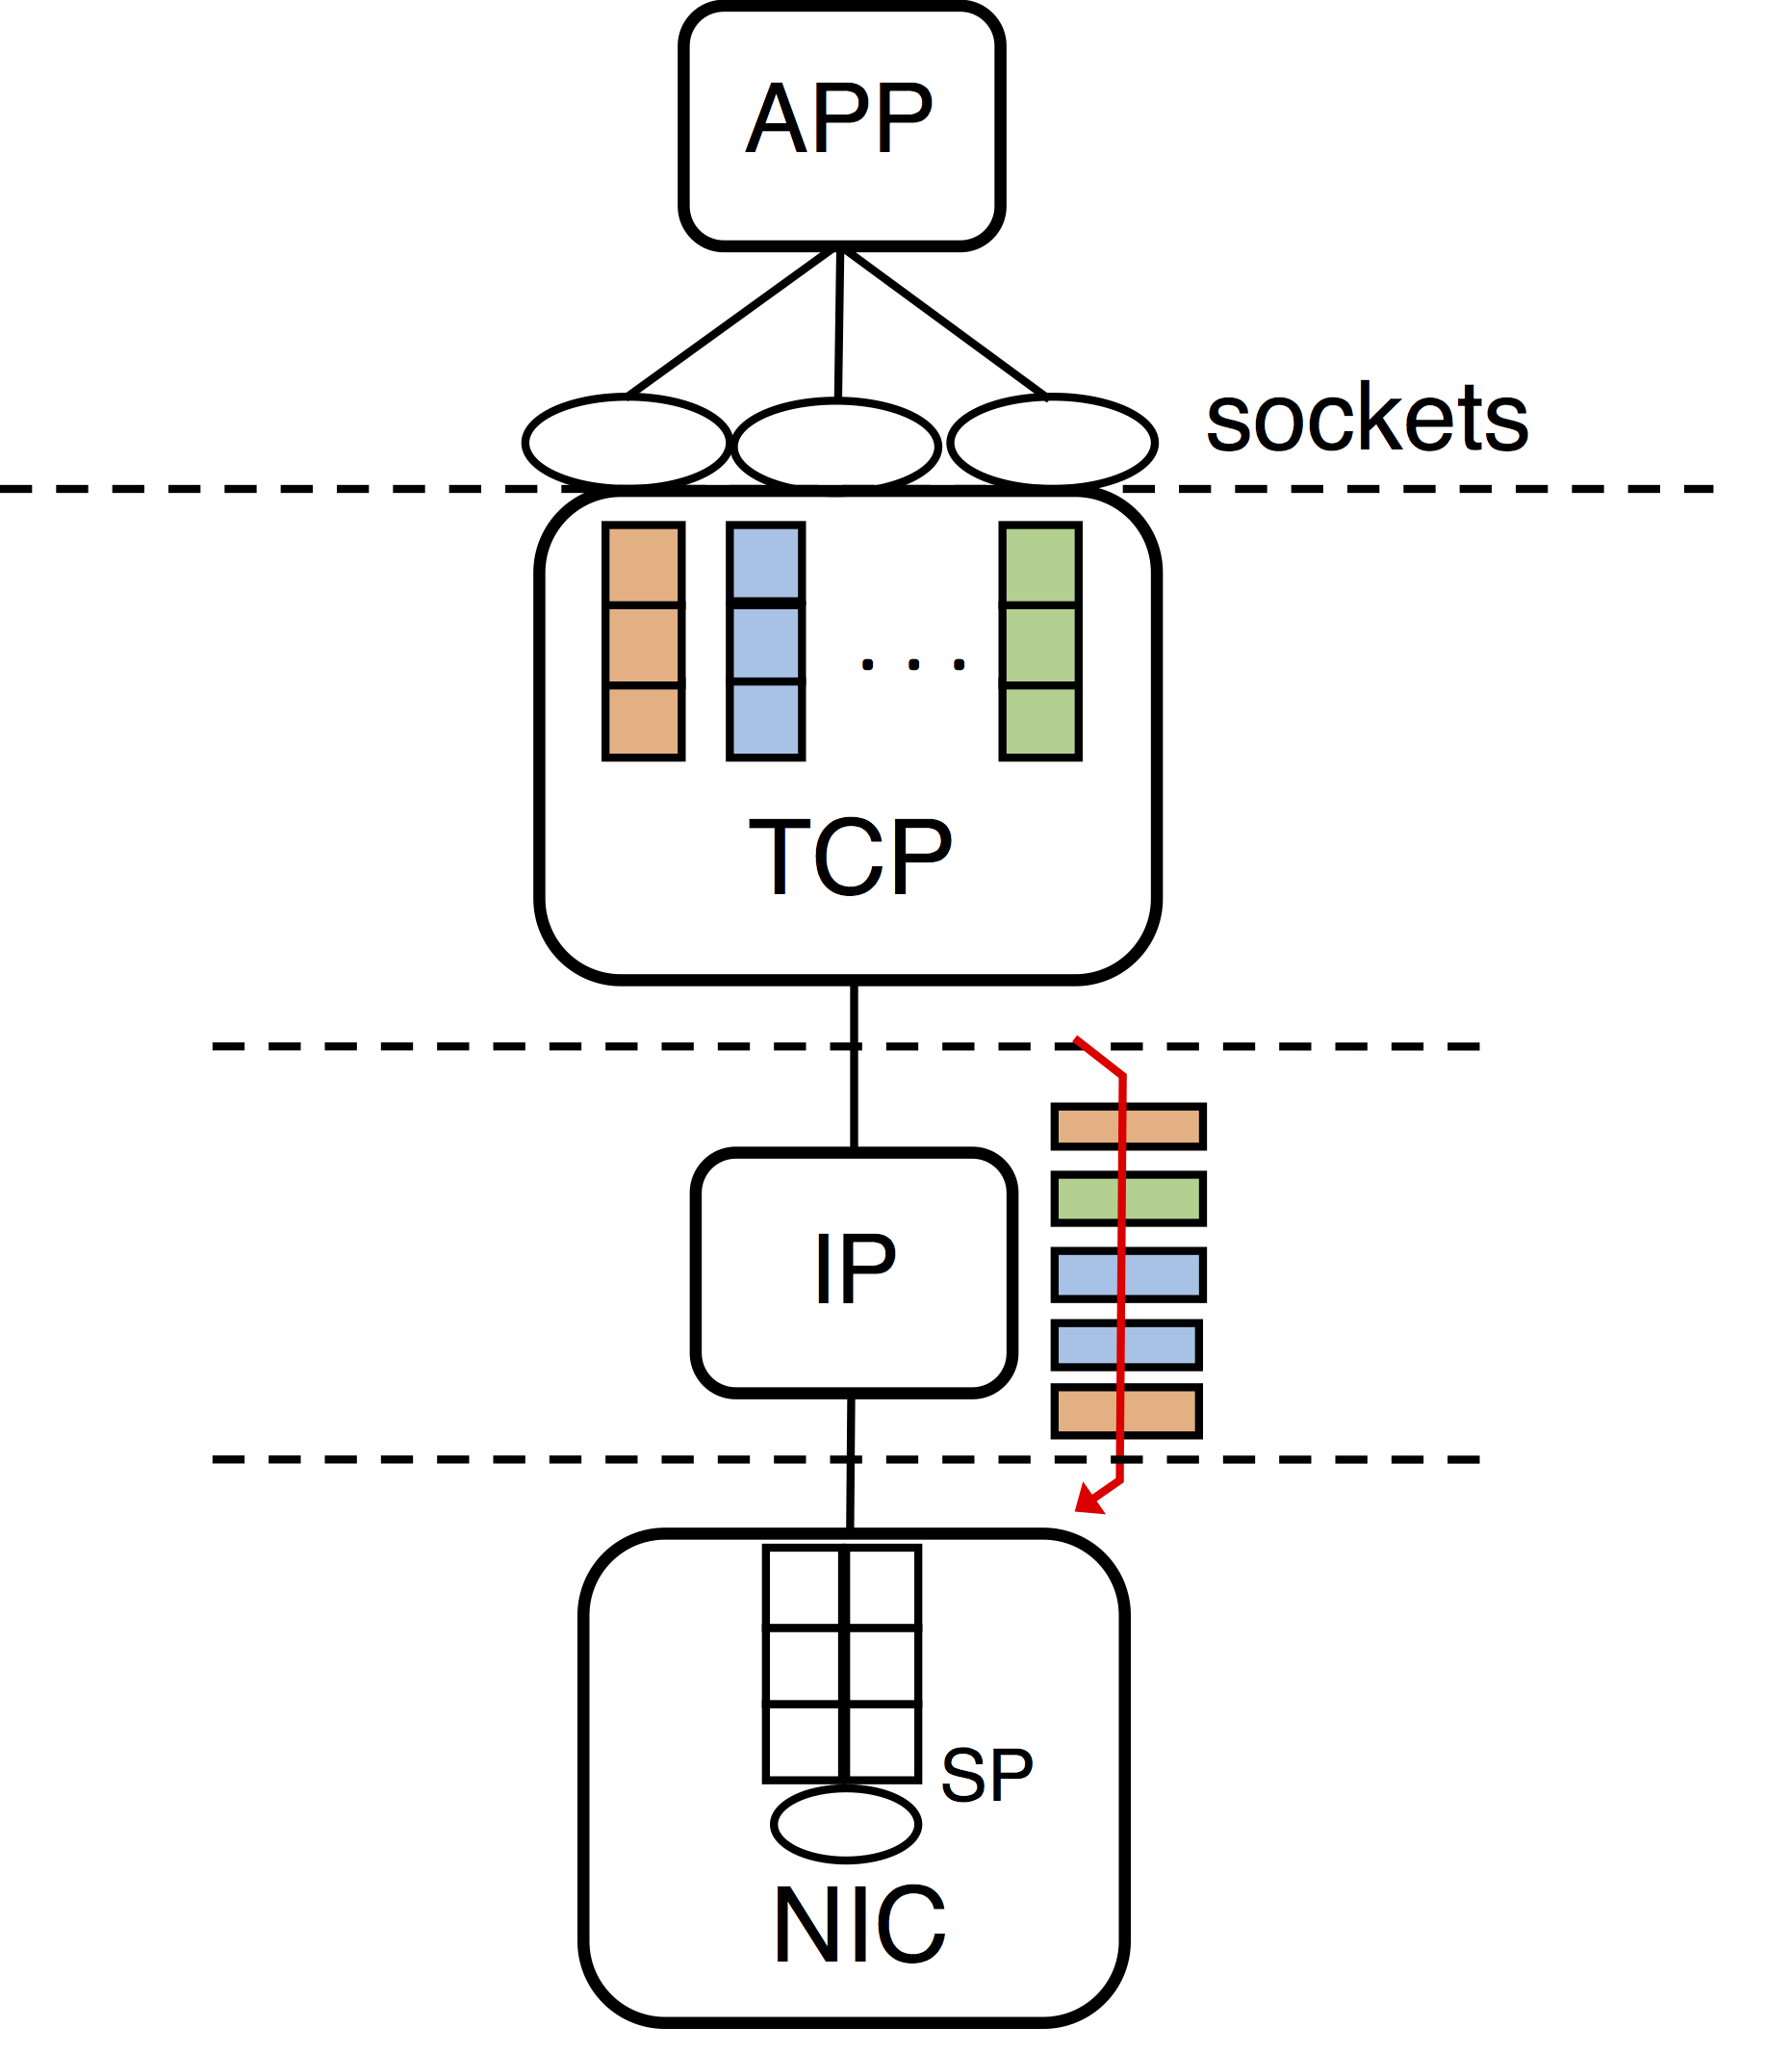
\includegraphics[width=0.4\linewidth]{Chapter4/Figures/tcp-config}
	\caption{Host architecture with TCP. Flows are interleaved thus emulating PS discipline.}
	\label{fig:tcp-config}
\end{figure}%
The architecture of the whole protocol stack at end hosts when adopting TCP is shown in Figure \ref{fig:tcp-config}. First start from the application layer. There is a unique application, following the generation process it setup a new TCP connection for each flow. Hence, already opened TCP sessions are not reused, but they are teared down when the flow completes. For every new connection, the application creates a socket, it batch sends the entire flow through the socket, offloading to TCP the segmentation in packets, then it immediately closes the socket. The application can close immediately the socket because it does not wait any data in response to its flow from the other peer of the TCP connection. There is not interaction, instead it only performs a one-way data transfer. For long flows this approach is not realistic. In a real TCP implementation the operating system would limit the maximum simultaneous bytes it can receive from the user application for preserving the memory allocation in kernel space. However, we can neglect these practical impairments to ease the implementation of the simulator. Opening and closing the socket in this way allows to avoid more complex management of simultaneous connection, like thread creation. Practically, our TCP application has been derived with some changes to the \texttt{TcpSessionApp} class of the standard INET library.\\
From the point of view of TCP, a separated transmission queue is allocated for each new socket. The simulator gave us the possibility to set the queue size limit to infinity. The scheduling among the queues is self-clocked by the TCP ACKs and transmission control mechanisms. A packet is popped from a queue only when the TCP window allow to do so. Simultaneous popping never occurs because ACKs belonging to distinct connections arrive back to back in the worst case. Therefore, packets of different flows are delivered to the IP layer with interleaving. When the socket transmission queue is completely drained, the TCP client immediately send a FIN packet for closing the connection, as the client application has already closed the socket. New connections always run the three-way-handshake during their setup and start with minimum window size. We do not set the initial window increase option of TCP. This is because the bandwidth-delay product of the network amounts to few packets. As a matter of fact, the distances between network elements in data centers are very short and propagation times on the network links are negligible for light speed. For example, on a link of 30m the bit propagation time is roughly 100ns. The transmission time of a TCP ACK packet on a 1Gbps link is 32ns. Thus, differently from large network on geographic scale, the Round Trip Time (RTT) is proportional to the packet transmission times. Since the topology is comprised by very few links, when multiplying the bandwidth and the RTT the result is near 5 packets.
We modified the defualt value of the TCP port range, in order to allow TCP to support the maximum number of simultaneous connection. With the default configuration, new connection could only use ports in the range 32768-61000. We extended the range to 1024-65535. Also, we removed the randomization of the initial sequence number, which is always started from zero. In this way, it is easy to discern the amount of service obtained by a flow and to tag its packets with the right priority. \\
Finally, we tackle at transport layer a possible shortcoming that has been also addressed in PIAS. Since we enforced strict priority queues also in the servers' NICs, that represent the first contention interface for the sender, large backlogs of packets may build up at end hosts. Indeed, the flows demoted to low priority stay active for long and many simultaneous flows share the server access link. They take time to converge to their fair share, meanwhile they increase their window to harvest additional bandwidth. The inet implementation of IP and MAC layer doesn't include back-pressure mechanisms to counteract the aggressiveness of TCP. Thus, either big delays or packet losses may be introduced yet before entering the network. A possible solution is to rate-limit to line rate the data flow between the application and the TCP. However, for the sake of simplicity we acted on the TCP Advertised Window (\texttt{AWND}) to upper bound the sender window to the bandwidth-delay product. Although the effect is practically the same, we are aware that in a real implementation the first solution is more clean. Indeed, the bandwidth-delay product of the topology is in general unknown or not specified to the servers. 
\subsubsection{UDP}
The scenario changes when adopting UDP as a transport protocol. Systems that aim to minimize the Flow Completion Time usually target transport protocols that ensure the delivery of the entire flow, thus neglecting UDP protocol. We tested the system also with UDP essentially for two reasons. First, it is easier to control its behavior, because it do not implement congestion control schemes, retransmissions, timeouts,..It is straightforward to check if the measured load on the topology corresponds to the offered load and verify the correctness of the traffic generation algorithm. Second, it may provide a rude approximation of the FIFO service at flow level, that gave the best results with spatial diversity (\S \ref{sec:dimensioning-spatial}). This is best understood considering Figure \ref{fig:udp-config}. It is well known that differently from TCP, UDP is connectionless. As a consequence, flows are packetized directly at application level and transfered to UDP already broken in datagrams. UDP does not have internal queues nor transmission control schemes, so it forwards all packets to IP, which in turn does the same with the MAC layer, that finally enqueues all packets in the line card buffers. In our simulator this happens in time zero, meaning that all these operations are code routines of the different layers that do not increase the simulation time. In other words, the new flow arrival event at application layer triggers all these network stack operations, which end only once all the packets of the flow are stored in the NIC's buffer. Since the simulator handles one event at a time, nothing else happens in the meantime. The relevant effect is that flows are served fully in FIFO order without interleaving at end hosts. In the network there is statistical multiplexing among different flows, even if the number of concurrent flows in the same interfaces is significantly reduced, due to the discipline enforced at the servers.\\
We use a trivial format for the application message, in order to make few information available on each UDP packet. In particular, we attach to application messages a sequence number and the flow length. Both the information are used for tagging packets with their priorities and to detect at the receiver when the flow is ended.
\begin{figure}[!tb]
	\centering
	\captionsetup{width=.75\linewidth}
	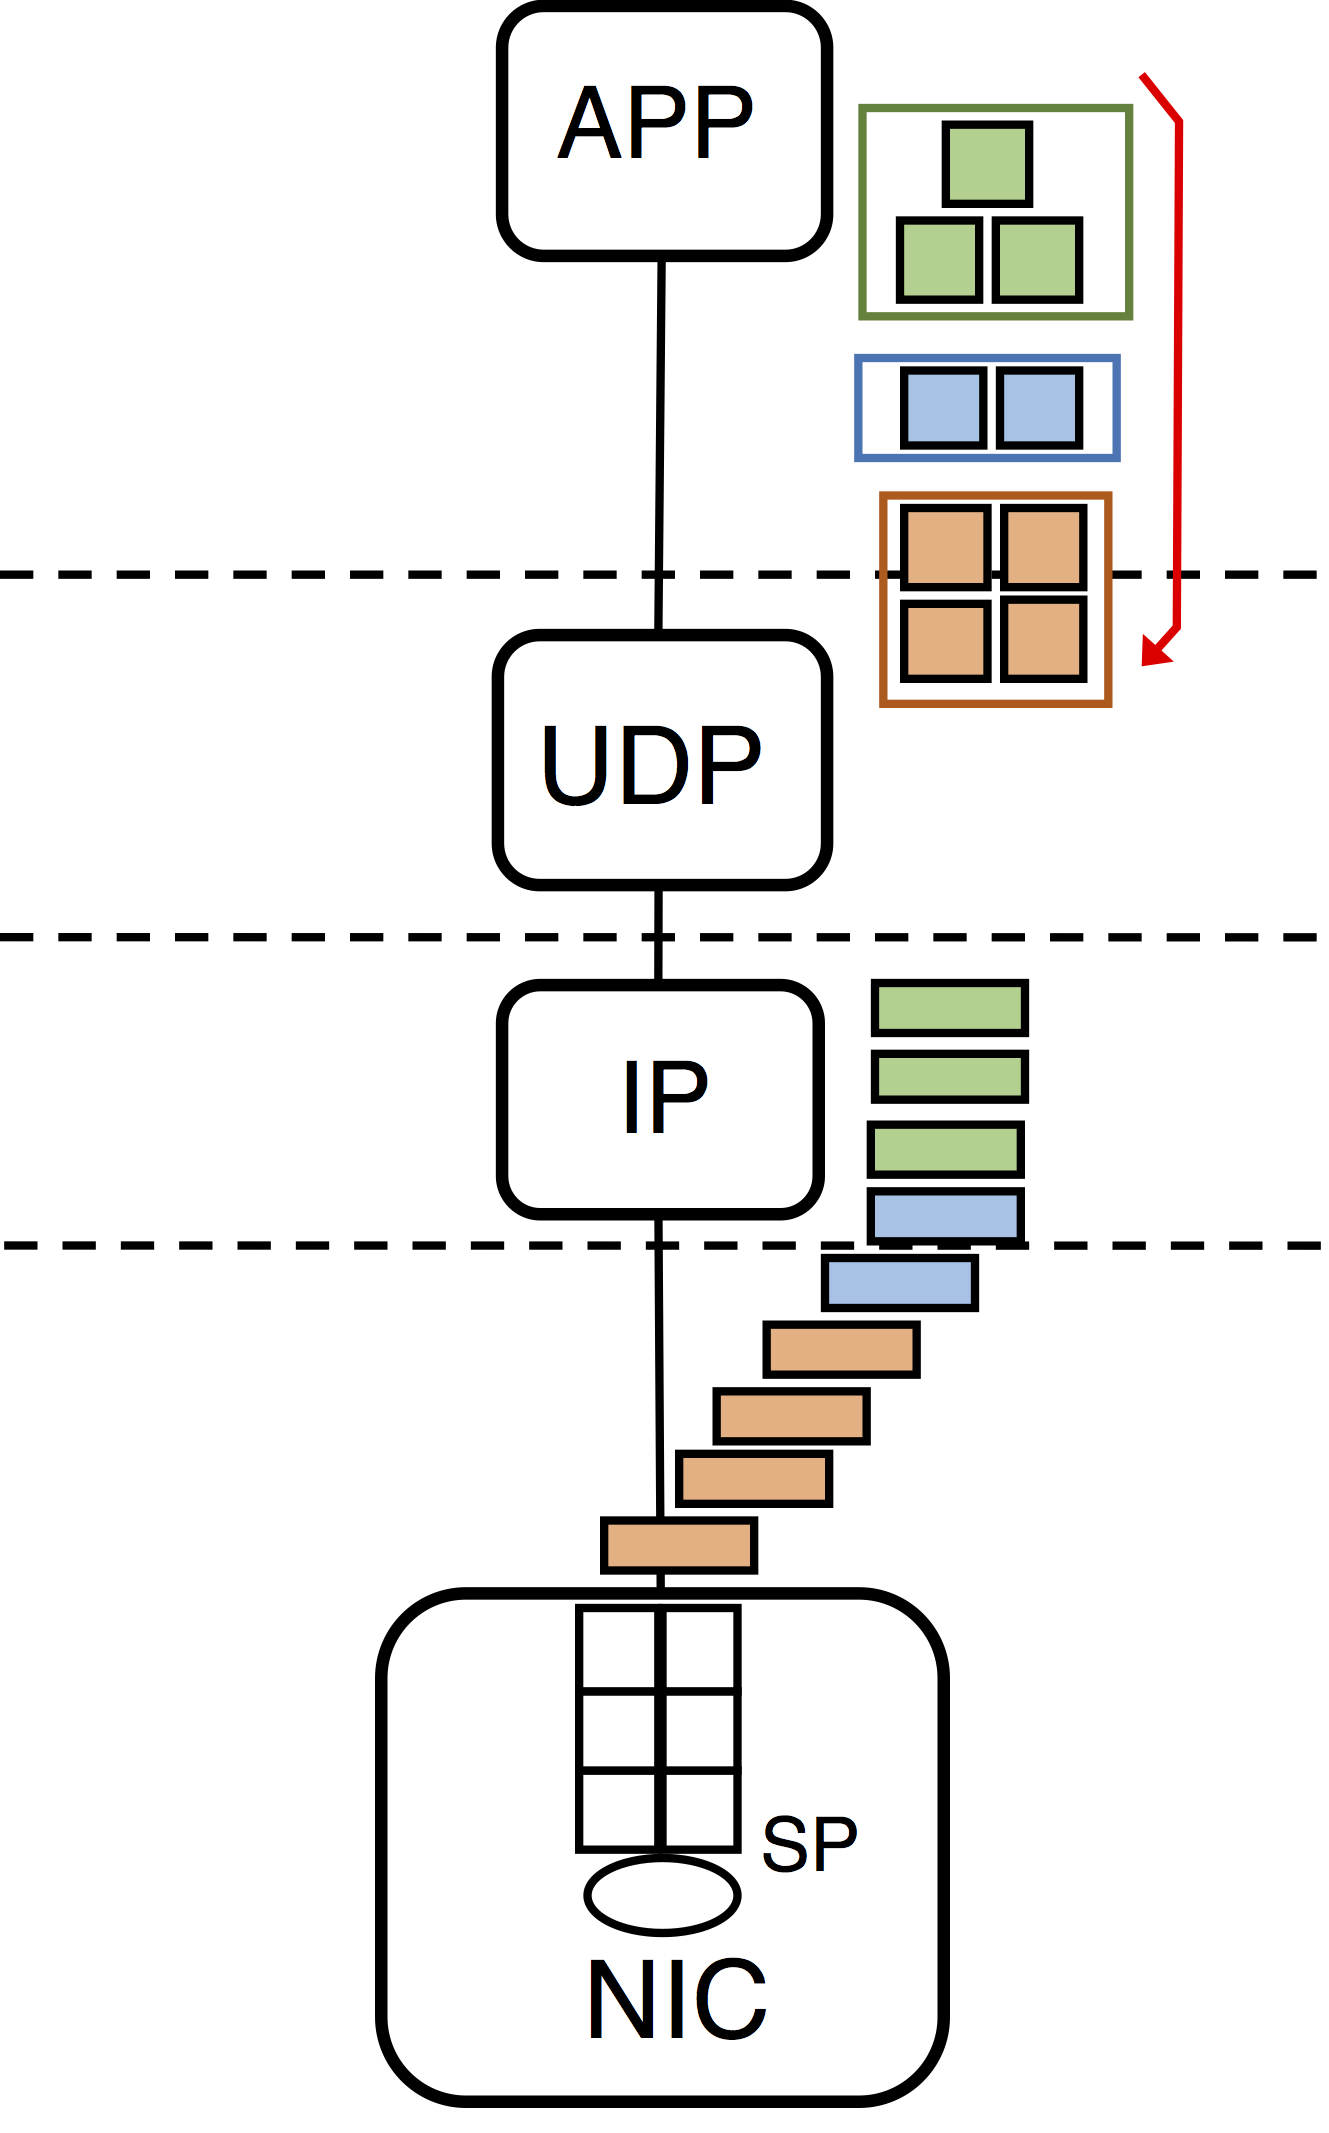
\includegraphics[width=0.3\linewidth]{Chapter4/Figures/udp-config}
	\caption{Host architecture with UDP. Flows are not interleaved thus emulating FIFO discipline.}
	\label{fig:udp-config}
\end{figure}%
\subsection{Network configuration}
% TODO modified djikstra
As discussed in chapter \ref{ch:sdframework}, a radical effect of SD-MLFQ is that the priority of a flow determines its routing over the topology. In a leaf-and-spine network, the ToR switches has to decide in which spine forward every packet, depending on some load balancing criterion. For SD-MLFQ, it is the flow priority, that has been assigned accounting for load balancing. Therefore spatial diversity has to be considered in routing algorithms. \\
We decided to handle the priority-dependent routing with a centralized controller module. End-hosts ask packet-by-packet to the central controller both the priority for their flows and the corresponding route. The controller knows the DC-wide flow size distribution and has computed all the demotion thresholds. Also, it keeps a centralized network view and it knows the priorities configured on every interface in the network. Thus, it can easily respond with a priority code and the route. The route depends on the load balance thresholds and it is provided as a vector of interface identifiers, whereas the priority code depends on the sub-thresholds. End hosts attach the interface IDs to their packets as a control information and tags the packets with the priority code. Finally, they send them through the network. The network devices use the interface identifiers for forwarding packets on the proper links and the priority to enqueue the packets on the proper priority queues. To sum up, it is applied a sort of source routing with the help of a central controller. \\
Both the route requests to the controller and the route information are handled offline, hence they don't contribute as overhead to network traffic. It means they are just data structures and function calls in the simulator. Instead, the priority code is carried in the DSCP field of the IEEE 802.1p \cite{ek1999ieee} standard for VLANs. This was the more immediate and flexible way to have a working prototype, without messing with solutions that make use of standard routing protocols to announce the priorities handled by the network nodes. The actual implementation of spatial diversity routing is out of the scope of this work. We think, however, that a centralized solution would be easy practicable also in modern SDN-based data center networks. \\
%Some changes were required to the inet modules in order to implement spatial diversity mechanism.
At this point, we built the entire topology using only standard inet modules for Ethernet switches with our modification for the forwarding-plane. We configured a single LAN for any topology size and we do not place any IP functionality inside the network. We do not need IP because the routing is handled by the controller. Also, we disabled the computation of the spanning tree and we instructed all servers with predefined entries in the ARP table before the beginning of the simulation. In this way we avoided all the possible problems that might arise from having a unique layer 2 network, such as spanning tree convergence or broadcast storms. Since we do not consider neither network nor server failures, the initial ARP mappings are valid for the entire simulation. We set priorities both at server and switch interfaces to implement the MLFQ scheduler. All priority queues are FIFO queues disciplined by a simple strict priority scheduler. Flow demotion is managed at the sources as explained above. Network switches are left with the only responsibility of choosing the priority queue by reading the DSCP code. \\
All links are Ethernet cables with a length of 30 meters, which seems reasonable in relation to the size of data center buildings. Buffer sizes are set to 1000 packets shared between priority queues of the same interface. Different ports have their own independent memories. We ignored switch architectures with port-shared memory pool, although they are common in data center networks \cite{dctcp, mqecn}.  In the experiments with UDP all queues have unlimited buffer space, in order not to loose packets and allow straightforward FCT measurements at the receiver. This is because packet losses would unnecessarily make controversial the meaning of FCT itself. Despite we are absolutely aware that the system with UDP has no practical value, nevertheless we recognize it has a theoretical utility.
\subsubsection{Priority assignment in down-send}
An aspect that we never addressed in the numerical simulator is how to assign priorities at the egress interfaces, that connect ToR switches to the servers. These ports are last traversed in the \emph{down-send} transmissions before leaving the switching fabric. During the up-send phase of the path from source to destination server we may exploit the spatial diversity to augment the priority classes proportionally to the number of spines. However, when traversing the egress interfaces all the priorities must be in some way mixed and multiplexed to the small number of queues available on a single port. This is illustrated in Fig. \ref{fig:downsend} for the case of rank=4 and two PQs per port, where 8 priorities have to be mapped on two queues. Our observation is that all egress interfaces receive the same DC-wide workload used for generating new flow sizes, because flows are uniformly sent to destination servers. Hence, we treat egress interfaces as in the system without spatial diversity, applying demotion at link level. In our experiments we mostly focused on 2 PQ, thus it was possible to compute rapidly the optimal PIAS threshold.
%\begin{figure}
%	\centering
%	\begin{subfigure}{.45\textwidth}
%		\centering
%		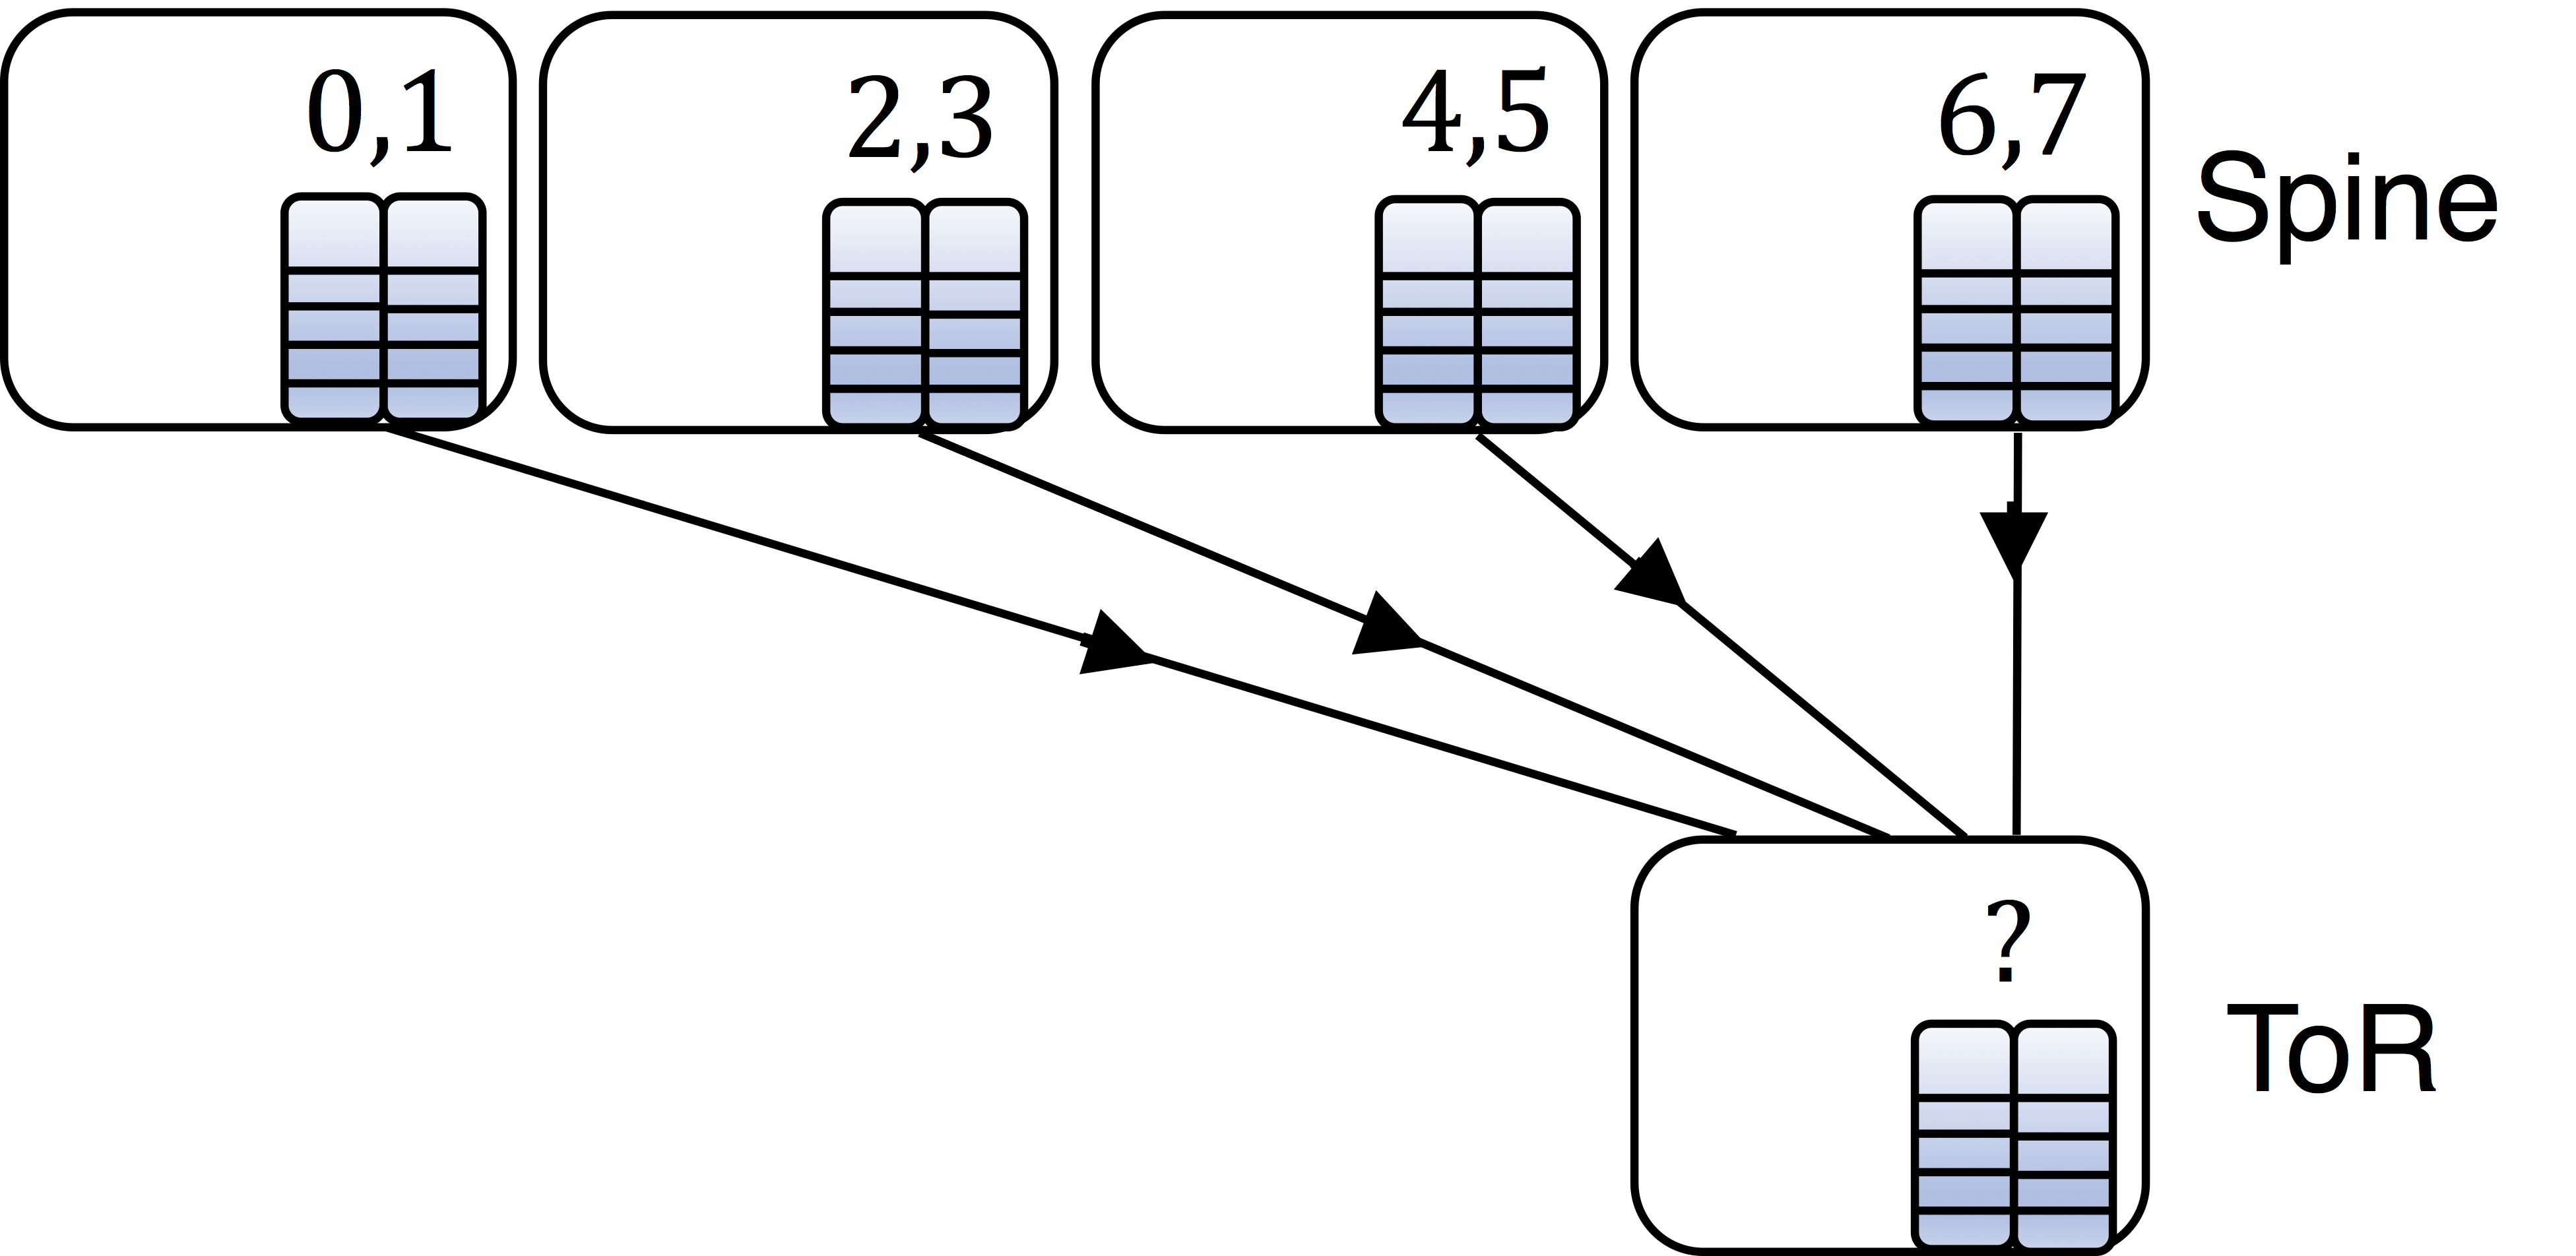
\includegraphics[width=0.99\textwidth]{Chapter4/Figures/downsend}
%		\caption{Example scenario}
%		\label{fig:example-downsend}
%	\end{subfigure}%
%	\hfill
%	\begin{subfigure}{.55\textwidth}
%		\centering
%		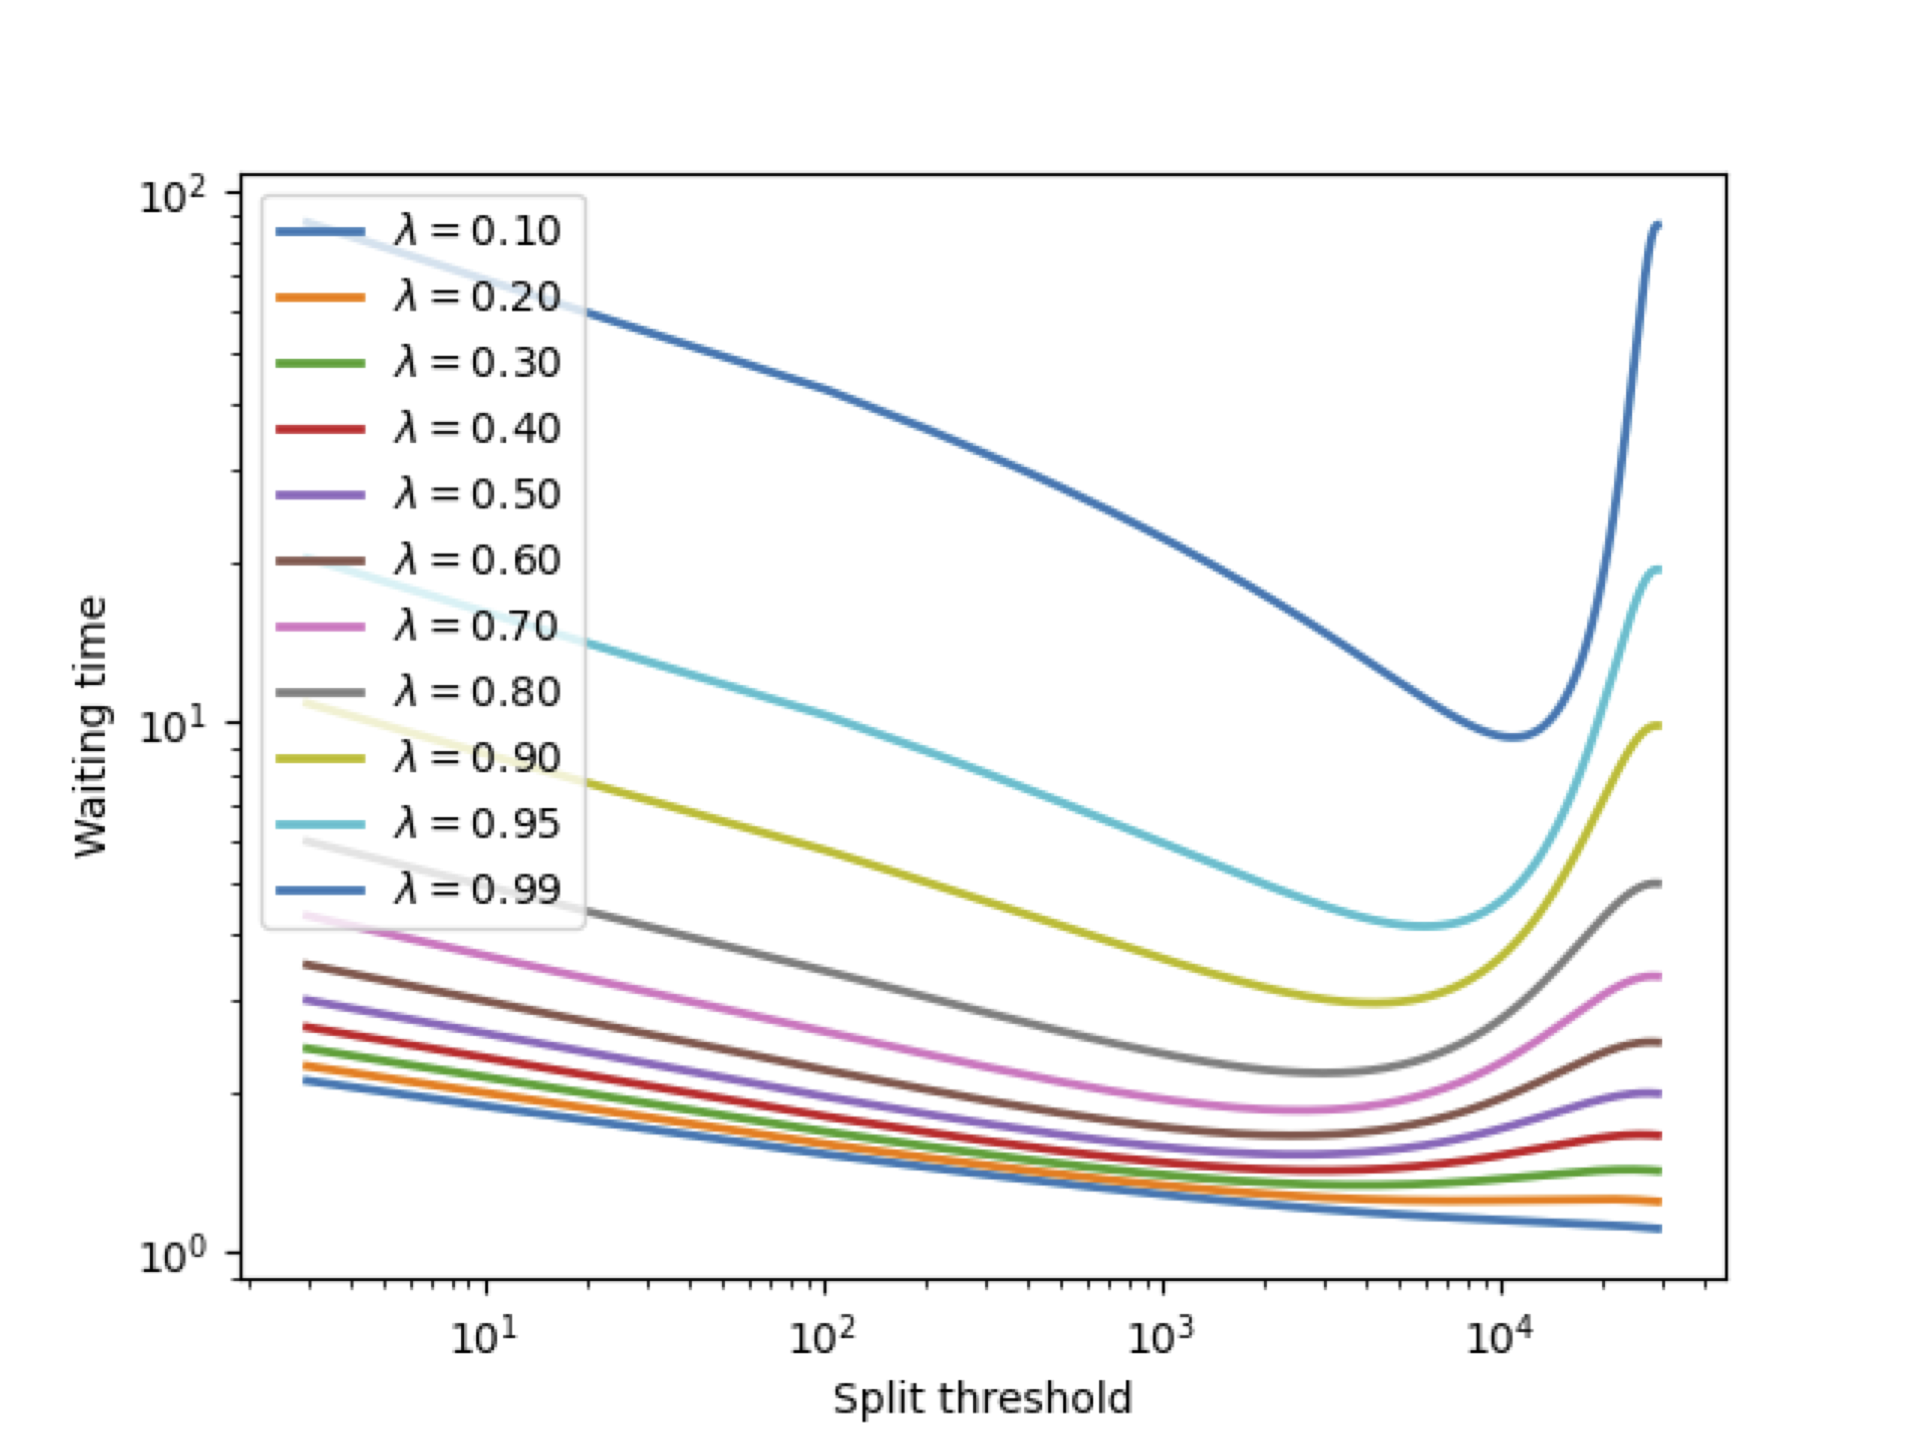
\includegraphics[width=0.99\textwidth]{Chapter4/Figures/opt-2pq}
%		\caption{PIAS thresholds}
%		\label{fig:opt-thresh}
%	\end{subfigure}%
%	\caption{Priority mixture in egress interfaces}
%	\label{fig:downsend}
%\end{figure}
\begin{figure}
	\centering	
	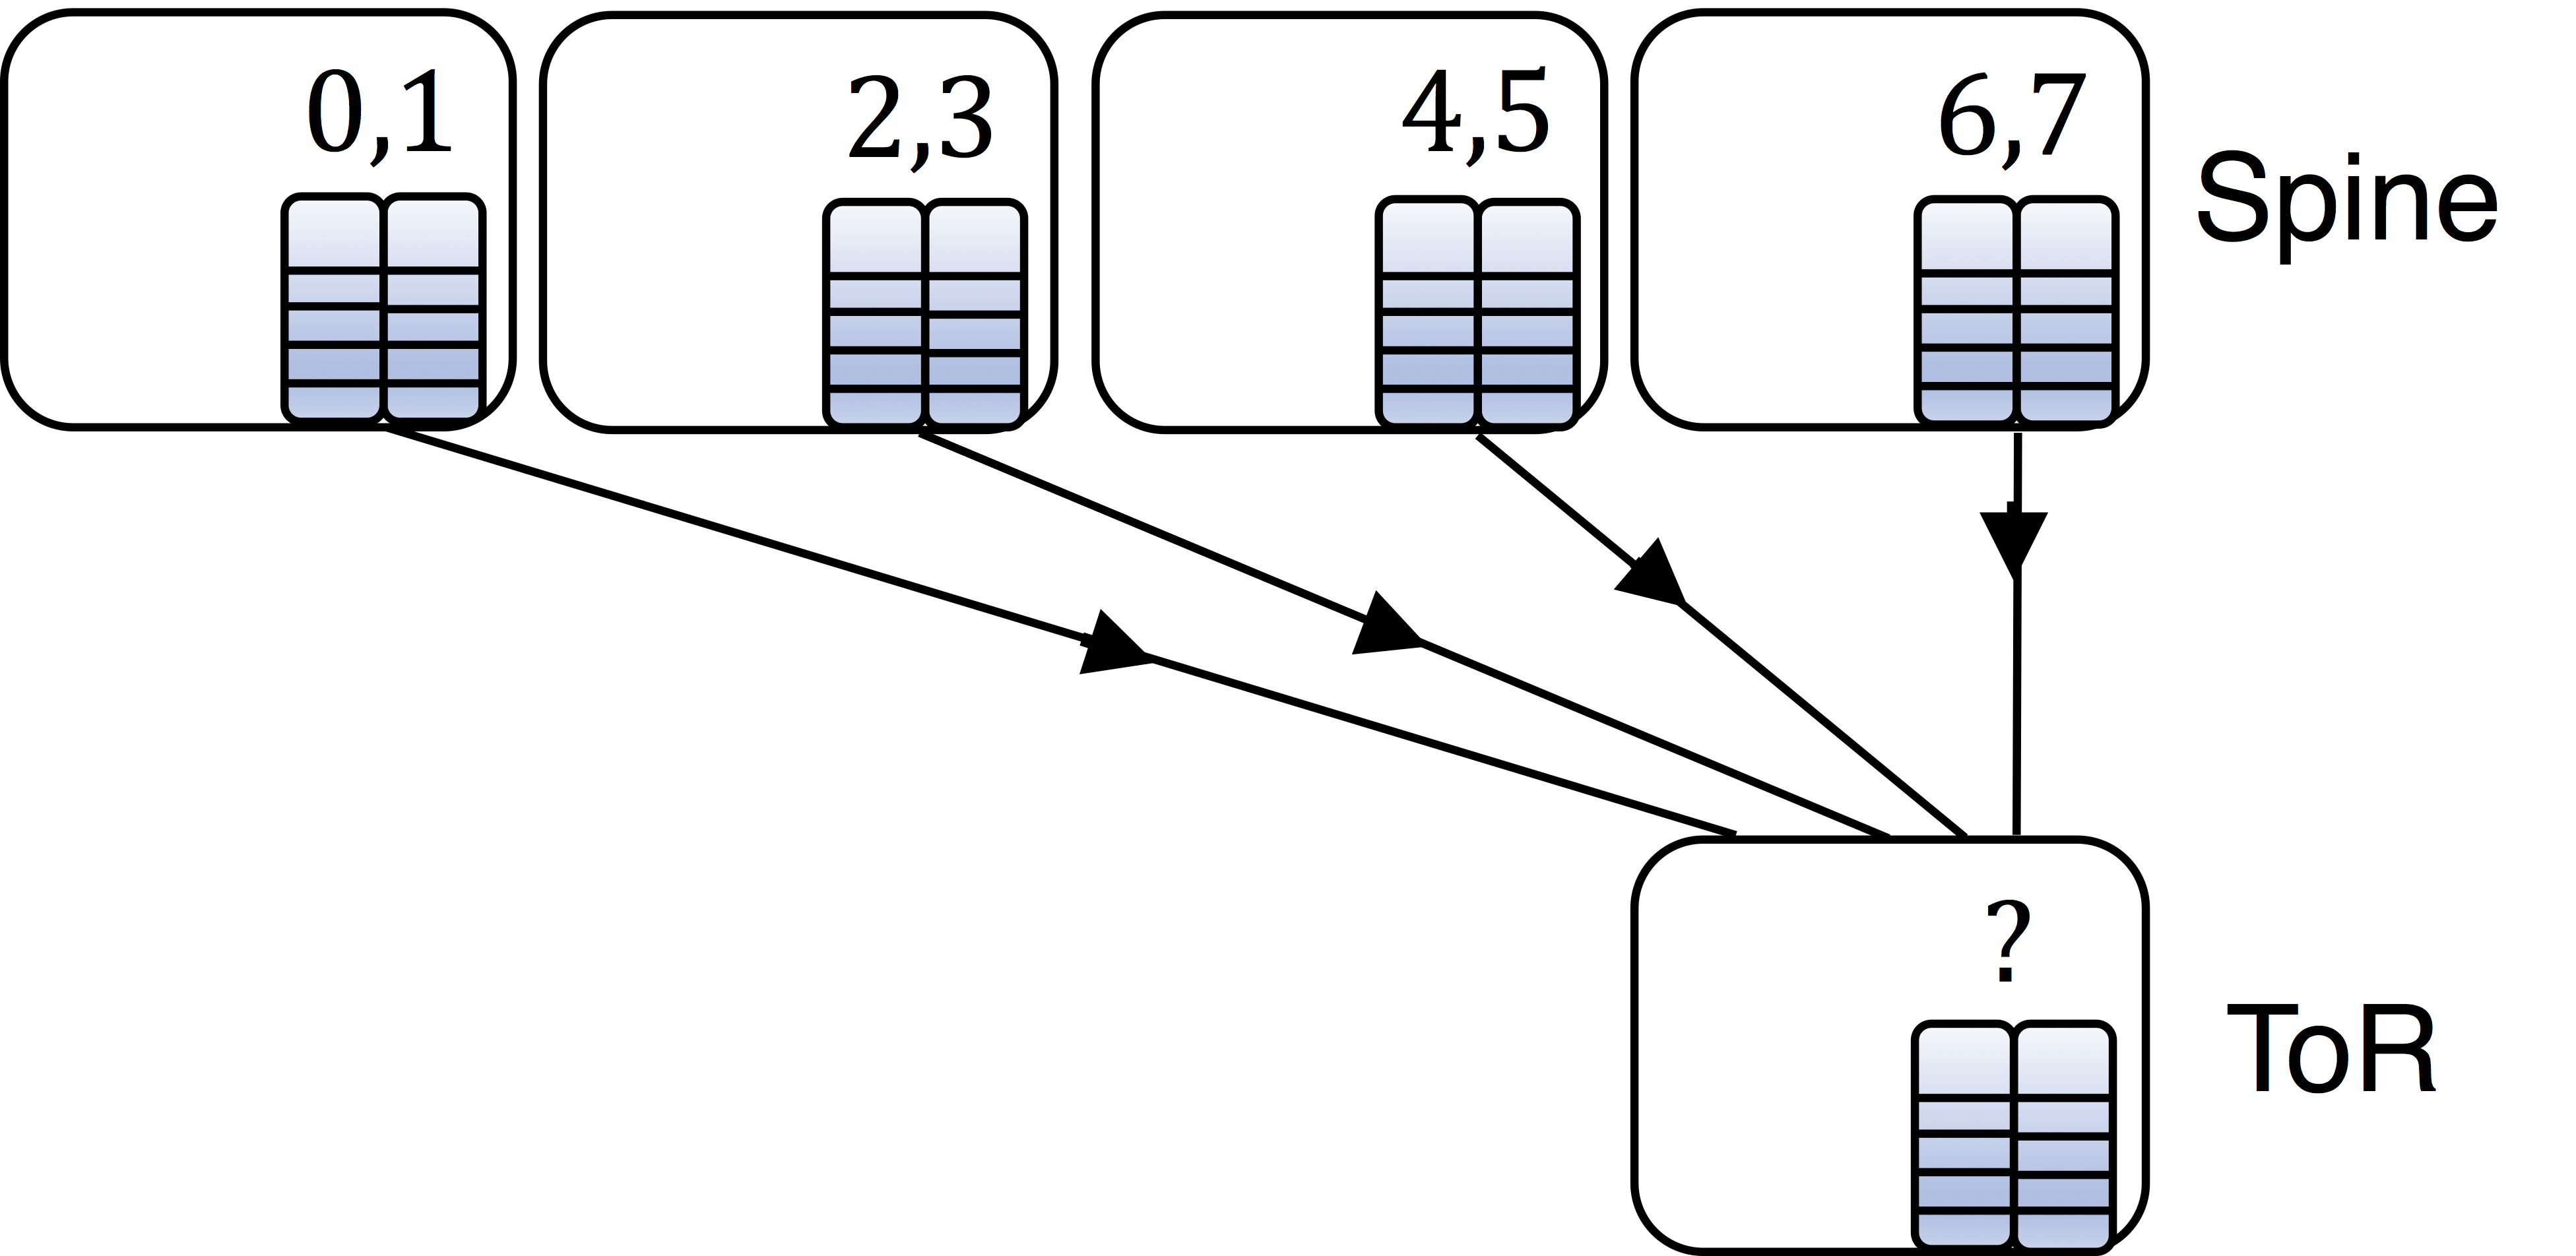
\includegraphics[width=0.5\textwidth]{Chapter4/Figures/downsend}
	\caption{Priority mixture in egress interfaces}
	\label{fig:downsend}
\end{figure}%
\subsection{Datacenter TCP(DCTCP)}
\label{sec:dctcp}
For the final versions of our experiments we employed state-of-the-art DCTCP \cite{dctcp}, among all possible versions of TCP.
Datacenter TCP (DCTCP) is a milestone for transport protocol design in data centers. It actually consists in minimal modifications to TCP New Reno. Its main insight is to leverage Explicit Congestion Notifications (ECN) from the network to properly modulate the window size of the TCP senders. The basic idea behind DCTCP is that queues in the network should be kept as empty as possible to avoid large backlogs that increase latency and do not leave enough headroom to absorb burst arrivals, occurring for example due to incast. Instead of pushing the window to grow until a packet drop is detected, the DCTCP transmitter slows down proactively depending on the level of congestion on the bottleneck link. Network queues mark packets with a congestion signal as soon they exceeds a given occupancy $K$. Then, TCP receivers convey back the congestion signals to TCP transmitters, setting the ECN-Echo bit to 1 in their ACKs. Finally, the TCP sender mantains an estimate $\alpha$ of the fraction of marked packet on an interval of roughly one RTT and modulates the window as:
\[ \text{cwnd} = \text{cwnd} \times (1-\alpha/2)\]
This way, upon mild congestion the window size is gently reduced --- note that only in case $\alpha$=1 it is cut in half as in standard TCP --- still ensuring high throughput, but mitigating its aggressiveness.\\It has been proven that DCTCP effectively succeed in lowering the amplitude of queue oscillations to $O(\sqrt{\text{BDP}})$, instead of $O(\text{BDP})$ of TCP, being BDP the bandwidth-delay product, while not losing throughput for a proper setting of the marking threshold $K$. More importantly, the queue length with DCTCP is proven to be predictable with an analytical expression. In the worst case of $N$ synchronized flows, the queue length is stable around $K+N$. \\
Note that the only requirement from the network is to configure switches with an AQM scheme to mark packets. In practice this can be achieved configuring the RED algorithm, already available in most devices, so that it marks based on the instantaneous queue length and with a unique high and low threshold equal to $K$. 
\subsubsection{DCTCP testbed}
We implemented the above changes to TCP in INET and the ECN markers to plug into the switch interfaces. We deployed the same testbed used in the original article of DCTCP \cite{dctcp}, in order to verify the correctness of the implementation. The testbed topology is shown in \ref{fig:dctcp-testbed-topology}. A group of $N$ server (on the left) start simultaneously long-lived TCP connections towards the same destination server (on the right). We used $N=2$ and $N=20$ and flow sizes fixed to TODO. All links are configured at 1Gbps speed and the DCTCP parameters set according to the guidelines of the reference paper. In particular, the threshold $K$ is set to 20 packets. \texttt{AWND} is set to its maximum value, so that the transmission control is not restricted. Buffer sizes are set to 500 packets.\\ %TODO check\\
\begin{figure}
	\centering
	\begin{subfigure}{.35\textwidth}
		\centering
		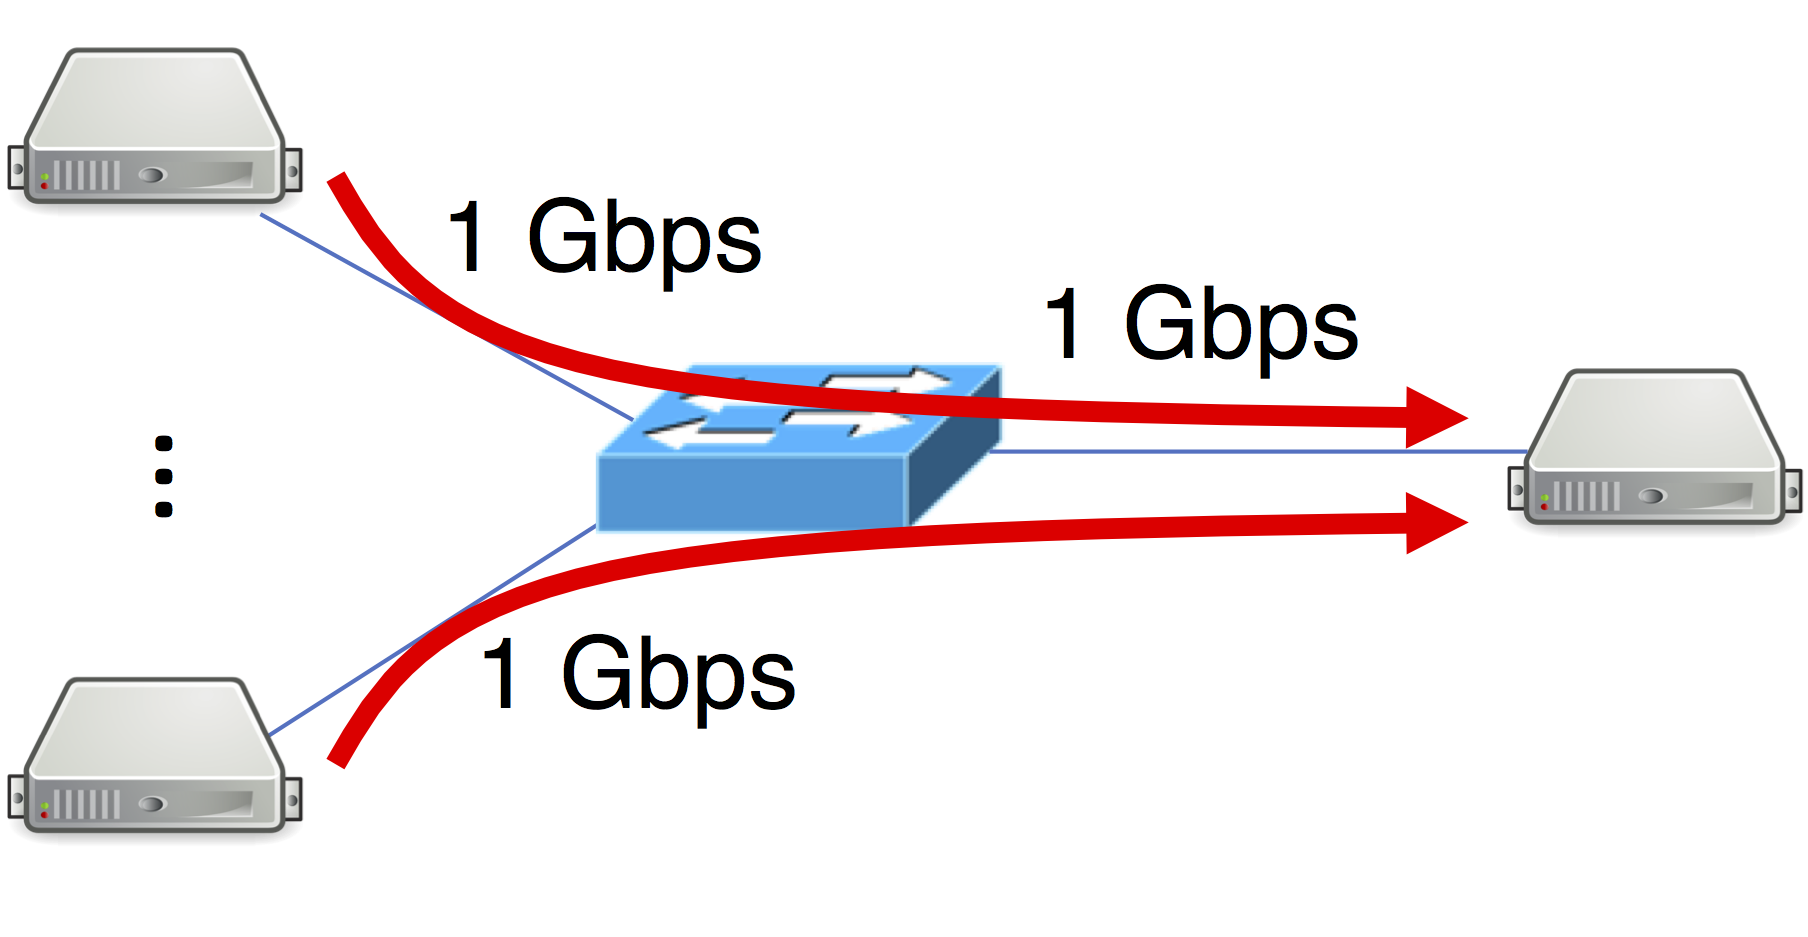
\includegraphics[width=0.99\textwidth]{Chapter4/Figures/dctcp-testbed}
		\caption{Testbed topology}
		\label{fig:dctcp-testbed-topology}		
	\end{subfigure}%
	\hfill
	\begin{subfigure}{.65\textwidth}
		\centering
		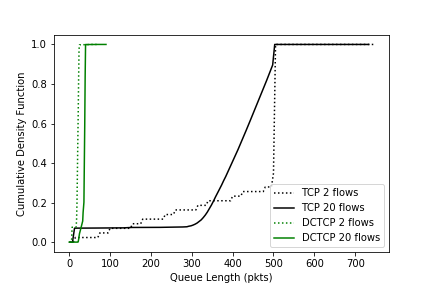
\includegraphics[width=0.9\textwidth]{Chapter4/Figures/dctcp-qlen}
		\caption{CDF of queue length, sampled every 3 packets}
		\label{fig:dctcp-testbed-res}		
	\end{subfigure}%
	\caption{DCTCP implementation testbed}
	\label{fig:dctcp-testbed}
\end{figure}%
We compare the CDF of the queue length when using TCP New Reno and DropTail queues in the bottleneck interface, with the case of DCTCP and ECN-enabled buffers (Fig. \ref{fig:dctcp-testbed-res}).  
It is clearly appreciable the effectiveness of DCTCP, which enforces the queue length to be stable around the predicted value. Conversely, with TCP DropTails the queue variance enlarges significantly, indicating the presence of large oscillations typical of sawtooth pattern induced by TCP AIMD congestion control scheme.
\subsubsection{Integrating ECN with SD-MLFQ}
We set ECN markers only in the network switches with recommended \cite{dctcp} threshold value. Conversely. servers have been equipped with simple DropTail queues and do not adopt AQM schemes. We dealt with few caveats in order to seamlessly integrate ECN rate control with the SD-MLFQ simulator. \\
\textbf{Per-port ECN marking}. First we had to choose how to apply ECN marking to the multi queue scenario. There are fundamentally two choices that trade latency, throughput and fairness. One possibility is to configure the recommended marking threshold independently on each of the $N$ priority queues available. This solution is known as per-queue ECN. It guarantees full link utilization in each priority queue, but the total queue length could potentially grow $N$ times larger and introduce high delays especially to low priority packets. Another option, referred to as per-port ECN, adopts a single marking threshold shared among different priority queues. While ensuring low latency, per-port ECN doesn't provide isolation among queues. Prior work \cite{mqecn} proposed dynamic threshold adjustment to provide best trade-off. We chose to simply use per-port ECN following the same approach as in PIAS. Per-port ECN could help in mitigating the long flow starvation problem. Starvation on low priority queues is undesirable with TCP, since it triggers retransmission timeouts of the connections even if the packets are not lost. Ultimately, it may lead to abrupt connection termination. With per-port ECN and its shared threshold, large buffer pressure on low priority queues helps in slowing down high priority traffic. \\ %TODO verify how many
\textbf{Marking \texttt{SYN/ACK} with CE codepoint.}
According to standardization \cite{ipecn}, ECN capable devices can mark with the congestion signal (\texttt{IP\_CE} - Congestion Experienced codepoint in the IP ToS field) only those packets with the  ECN Capable Transport codepoint set (\texttt{IP\_ECT} codepoint). However, the standard ECN extension to TCP specifies that control packets (\texttt{SYN, ACK, FIN},.) must been transmitted as Non ECN-Capable (\texttt{IP\_NOT\_ECT} codepoint). Thus, if they enter a switch interface when its occupancy exceeds the marking threshold, they are dropped rather than being marked. We noticed in our first simulations with DCTCP an anomalous number of retransmission timeouts (RTOs). We better investigated the number of bytes transmitted when TCP connections experienced RTOs: practically all timeout events occurred at connection setup. Thus, we implemented the modification to TCP that allows ECN-Capable control packets \cite{synecn}.
\section{Result analysis}
